\documentclass[a4paper]{article}
\usepackage{xeCJK,fontspec, booktabs}

\usepackage{fancyhdr,indentfirst}
\usepackage[left=31.8mm,right=31.8mm,top=25.4mm,bottom=25.4mm]{geometry}
\usepackage{graphicx,color,xcolor,xecolor}

\setmainfont[ItalicFont={LXGW WenKai}]{Source Han Serif SC}
\setCJKmainfont[ItalicFont={LXGW WenKai}]{Source Han Serif SC}
\setsansfont[ItalicFont={LXGW WenKai}]{Source Han Sans SC}
\setCJKsansfont[ItalicFont={LXGW WenKai}]{Source Han Sans SC}

\xeCJKDeclareCharClass{CJK}{`①,`②,`③,`④,`⑤,`⑥,`⑦,`⑧,`⑨,`⑩,`⑪,`⑫,`⑬,`⑭,`⑮,`⑯,`⑰,`⑱,`⑲,`⑳,`☆,`★,`○,`●,`□,`■,`♂,`♀,`◇,`⋯}

\usepackage{pdfpages,hyperref}
\usepackage{tabularray}
\usepackage[normalem]{ulem}
\usepackage{amsmath, amsfonts}

\hypersetup{
    colorlinks,
    linkcolor=black,
    pdftitle={北邮沙河生存手册R},
    pdfauthor={北邮软件工程根据地\ 群}
}

\DefTblrTemplate{caption-tag}{normal}{表}
\DefTblrTemplate{contfoot-text}{normal}{续下页}
\DefTblrTemplate{conthead-text}{normal}{续表}
\SetTblrTemplate{caption-tag}{normal}
\SetTblrTemplate{contfoot-text}{normal}
\SetTblrTemplate{conthead-text}{normal}

\newcommand{\faq}[1]{\subsubsection*{#1}}
\renewcommand{\contentsname}{目录}
\renewcommand{\baselinestretch}{1.25}

\begin{document}

\includepdf{cover.pdf}

\begin{titlepage}
    \centering
    \vspace*{\stretch{1}}
    {\Huge\rmfamily\bfseries 北邮沙河生存手册R} \\[6.5ex]
    {\Large\sffamily 北邮软件工程根据地\ 群} \\
    \vspace{\stretch{3}}
    {\large\ttfamily v3.0.0, July 2023}\\[1.5ex]
    \vspace{\stretch{0.5}}
\end{titlepage}

\newpage
\begin{center}
\section*{声明}

本作品由“北邮软件工程根据地\ 群”的群友集体创作。\\
可以在\href{https://github.com/BUPTSE/welcome}{此}获取本文档的源代码。

\smallskip

本内容以“CC BY-SA 4.0”许可证共享。要查看该许可证,可访问\\
\href{https://creativecommons.org/licenses/by-sa/4.0/}{https://creativecommons.org/licenses/by-sa/4.0/}

\smallskip

受相关政策变化影响,部分内容可能有失准确,请以学校方面要求为准。

\bigskip

\end{center}

\newpage
%\raggedright
\setcounter{page}{1}
\tableofcontents

\newpage
\setcounter{page}{1}

\pagestyle{fancy}
\lhead{\small \leftmark}
\chead{}
\rhead{\small 北邮沙河生存手册R}
\lfoot{}
\cfoot{\thepage}
\rfoot{}
\renewcommand{\headrulewidth}{0.4pt}
% \renewcommand{\footrulewidth}{0.4pt}

% 1.新生报到
\section{新生报道}

\subsection{学号与班号}

首先欢迎2023级软件工程的同学们加入这个豪华\sout{孤儿院}大家庭!

当你正式来到北邮的时候,便会得到两串十位数字:学号和班号。我们依次解读:
\begin{itemize}
    \itshape
    \item 学号:2023(年份)21(全日制本科生)XXXX(四位学生编号)
    \item 班号:202321(同上)13(计算机学院\footnote{计算机学院(国家示范性软件学院)})15/16/17/18/19(软件工程的五个班\footnote{软工的班级和计算机类混编为三大班})
\end{itemize}

接触许许多多的新账号时不必头疼,优先尝试账号为学号,密码为身份证后6/8位或者8位生日的组合,能解决80 \%的问题。(注意,身份证号含有X的需要大写或者替换为0。)

例如:教务系统的初始密码为8位生日,校园卡的支付密码是身份证号后六位。

\subsection{报到流程}

报到的具体流程,在学校发放的新生手册中有详细介绍。通常来讲,大概分为宿舍入住、报到登记和一卡通办理等部分。这几部分一般没有顺序要求,强烈建议首先完成宿舍入住手续的办理,把行李丢在宿舍以后再去办其他手续会方便不少。

报到当天会有志愿者在北京站、北京南站、北京西站给坐火车的同学们接站,到学校以后也会有志愿者(就是学长们啦)全程接驾,千万不要紧张哦(


% 2.校区环境
\section{校区环境}

北邮现在使用中的校区一共三个,即西土城路校区(海淀区,本部)、沙河校区(昌平区)以及海南校区(仅限玛丽女王海南学院)\footnote{另有西城区小西天校区(校舍)和昌平区宏福校区(接近弃用),目前和大家关系不大,唯有实验课偶尔会去一两次。}。

校本部位于海淀区西土城路10号,面积很小,住宿条件相对较差,但交通便利,对面就是北师大,周围美食众多。目前,大部分大三大四的本科生及多数研究生在本部学习。沙河校区是新生入学的校区,位于昌平区沙河镇南丰路1号,规划面积很大(大概本部三倍)但是实际只建成规划面积的一半多;住宿学习环境好,但比较偏僻,出行不便。

除海南学院外的所有新生都将在沙河校区入学并在这至少读完大一。

\begin{center}
    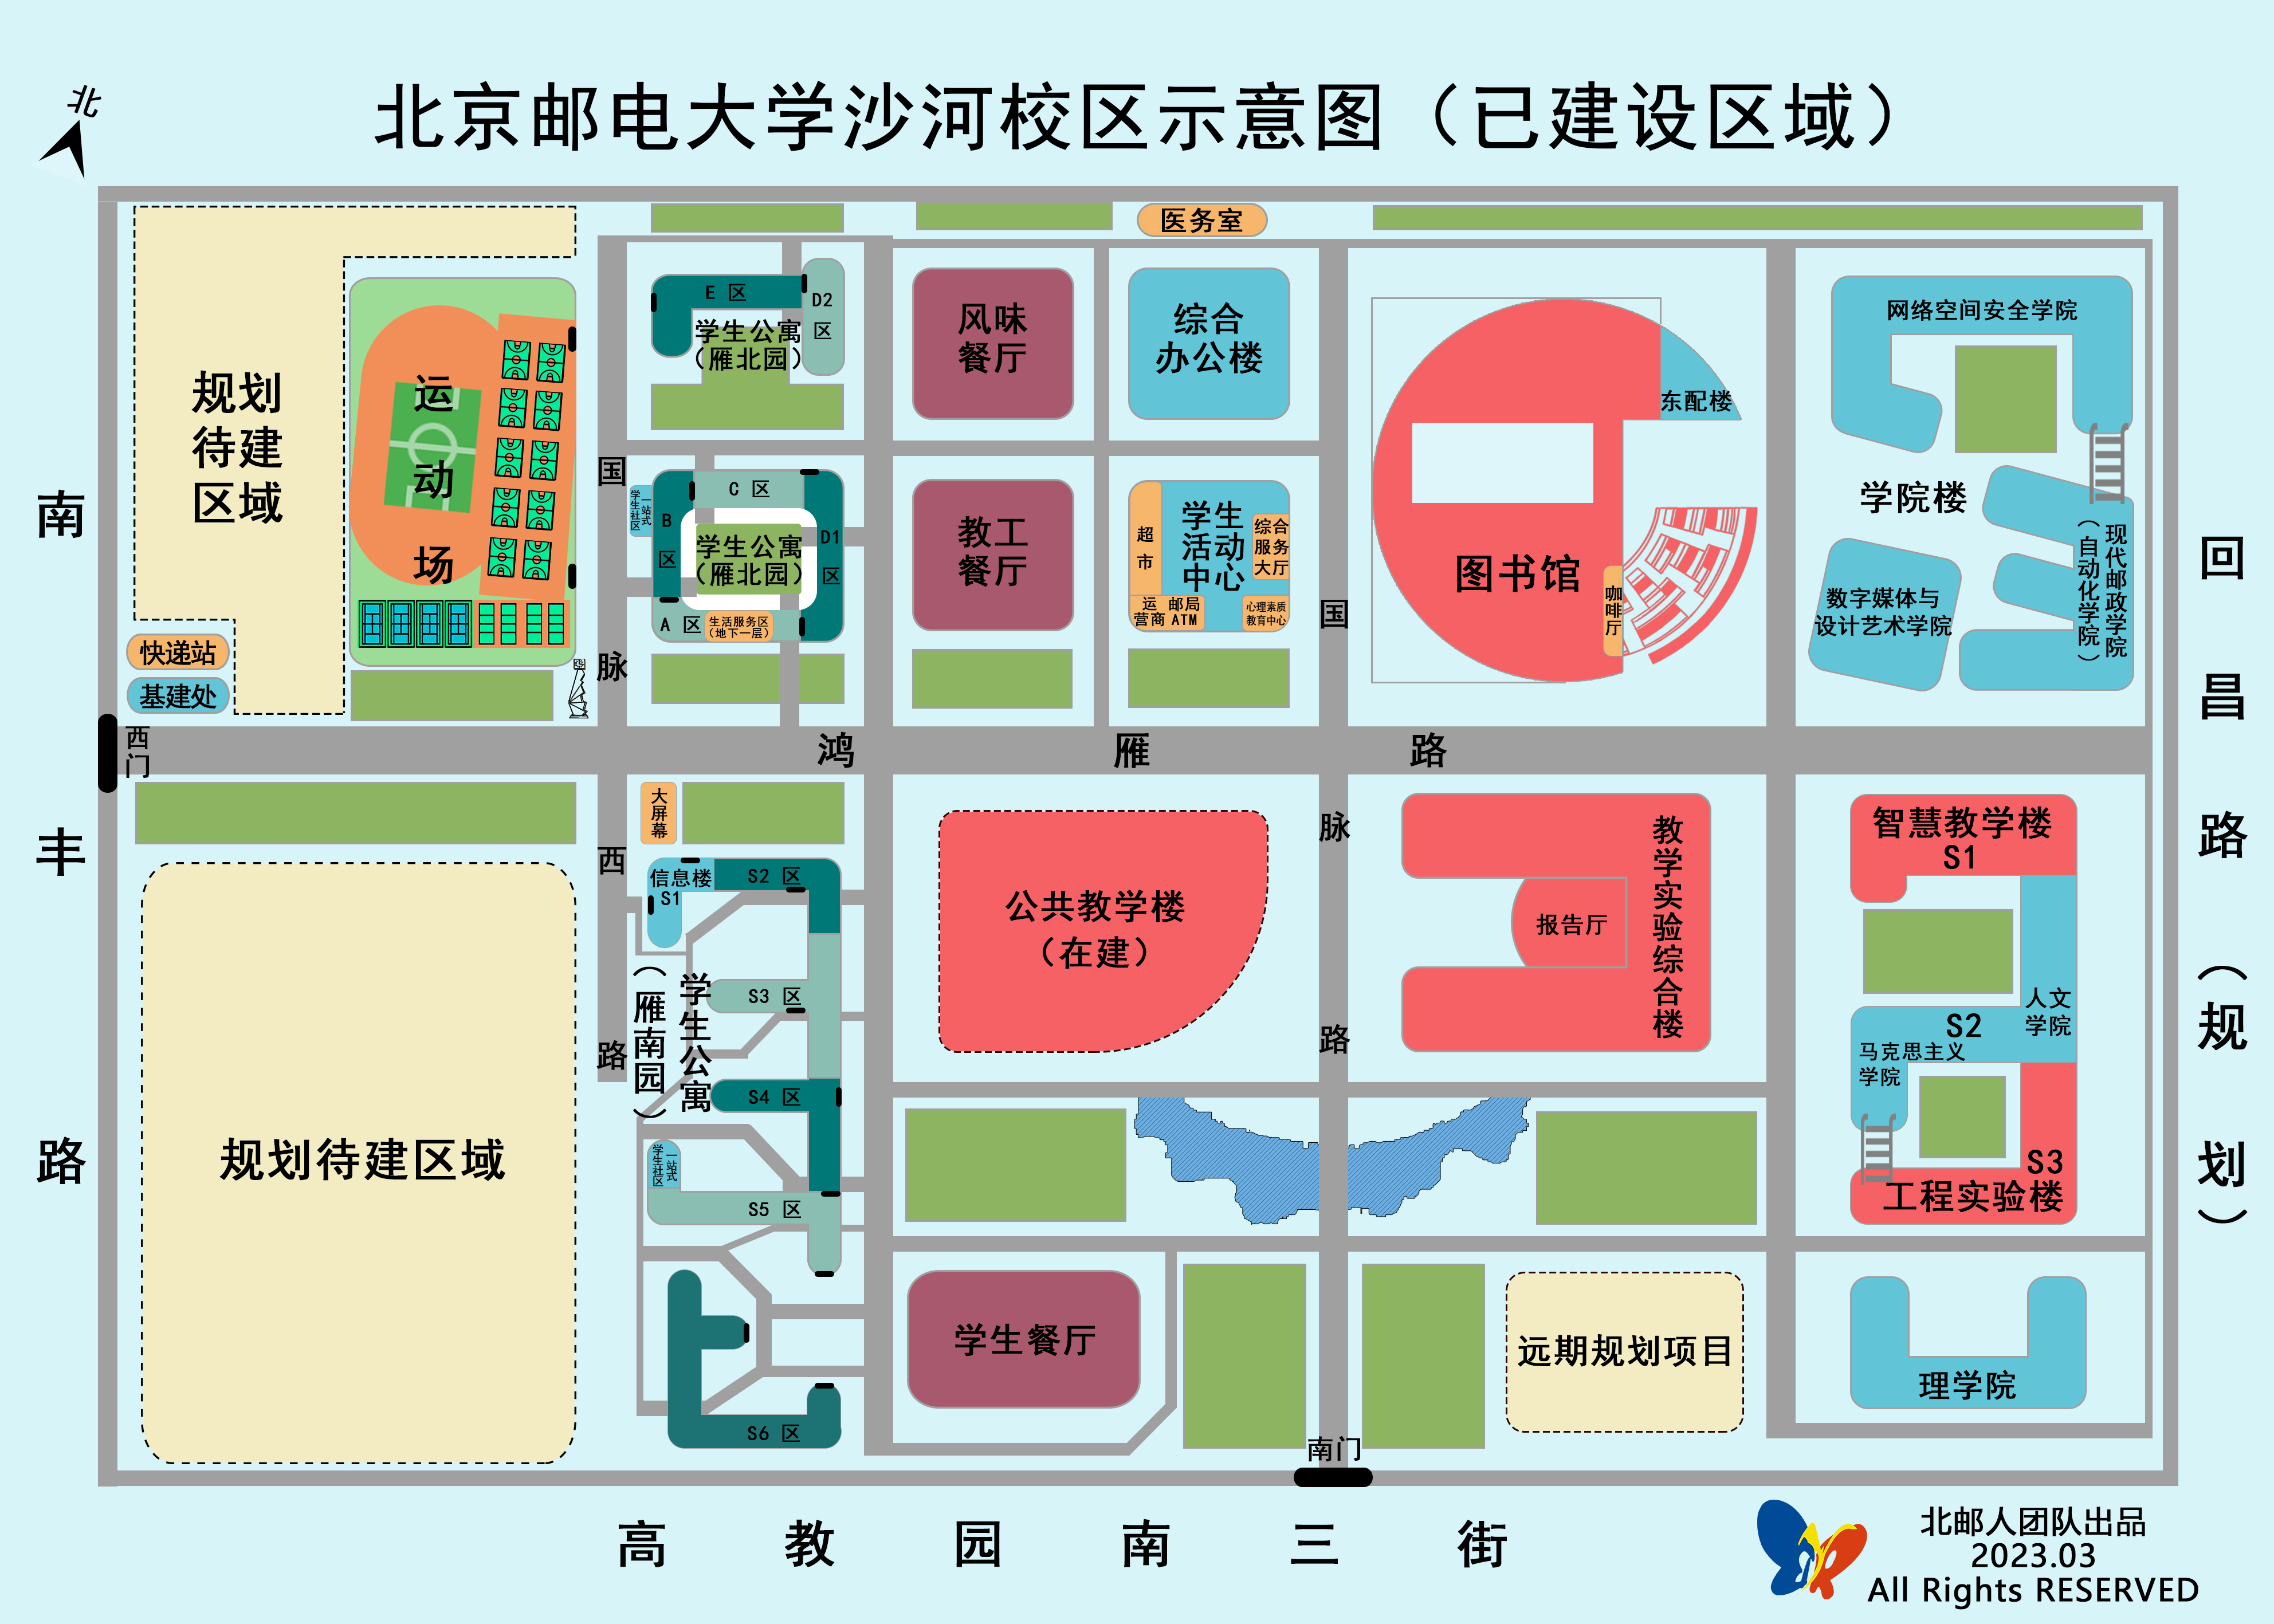
\includegraphics[width=0.80\textwidth]{images/shahe-map.jpg}
\end{center}

\faq{校园到底有多大?绕一圈要多久?}

很小,真的很小。本部绕一圈仅需10分钟,沙河大概也就20分钟。{\small (不过小也有小的好处,比如说可以7:55起床去上8:00的课。)}

\faq{我什么时候会从沙河搬到本部?}

按照学校最新的安排,各个学院的本科生从沙河搬到本部的时间如下表:

\begin{center}
    \begin{tabular}{cc}
        \toprule
        学院 & 搬迁时间(学年开始) \\
        \midrule
        计算机学院(国家示范性软件学院) & 大二 \\
        经济管理学院 & 大二 \\
        国际学院 & 大二\\
        信息与通信工程学院 & 大三 \\
        电子工程学院 & 大三 \\
        人工智能学院 & 大三 \\
        \bottomrule
    \end{tabular}
\end{center}

网络空间安全学院、现代邮政学院(自动化学院)、理学院、人文学院、数字媒体与设计艺术学院不搬至本部(即在沙河校区读完本科四年)。未来学院是否搬至本部、哪学年搬尚不确定。

除参照上表外,学校已经在\href{https://zsb.bupt.edu.cn/info/1005/1992.htm}{招生章程}中写出了各专业的办学地点。

\faq{沙河校区距离地铁站远吗?是几号线?}

沙河校区附近有两个昌平线地铁站,往南一公里是沙河站,往北七百米是沙河高教园地铁站。沙河校区被这两个站夹在几乎正中间,导致出行不是十分方便。

地铁昌平线沙河站-西土城站区间加上学校和地铁站之间骑车的时间一共需要60-70分钟(不含地铁等车时间),沙河站附近商铺较多,但沙河高教园站乘车人数与沙河站相比会相对较少,实际乘坐时间几乎没有差别。

\faq{有校车吗?免费吗?}

有,校车往返本部和沙河,并且是免费的。学期开始后可以在学校后勤处的公众号“北京邮电大学后勤处”中查看具体班次。校车正常情况下单程用时35-55分钟(不含等车时间)。

沙河校区在图书馆十字路口处靠学生活动中心路北登车,本部在教三楼西侧登车。由于校车要优先服务教师职工,加之高峰时段乘车需求众多,建议提前20分钟到指定地点排队等待。

\faq{寒暑假我可以住在学校吗?}

可以住在学校,但由于本科生从沙河校区搬往本部是在新学年开始时进行,所以下一学年搬往本部的同学,暑假只能住在沙河校区。


% 3.住宿条件
\section{住宿条件}

\subsection{沙河宿舍简介}

根据宿舍楼的位置,沙河校区的宿舍分为雁北园和雁南园。相对而言,雁北园的条件会差一些,比如阳台空间较小、公共浴室较为破旧和储物空间较少。但其实也只是差一点(

\emph{雁北园}位于鸿雁路北侧,各区域的代号为A/B/C/D1/D2/E,离两个食堂\footnote{教工餐厅、风味餐厅}、操场、生活服务区较近。A/B/C/D1是四栋矩形相连的宿舍楼(一楼入口独立,二楼以上的部分相连),其中C与D1入口有电梯,而A与B入口没有;D2/E是另两栋在更北侧独立于A/B/C/D1宿舍楼且相对较小的宿舍楼,内部也是相连的。

\emph{雁南园}位于鸿雁路南侧,各区域的代号为S2/S3/S4/S5/S6(S1是信息中心楼),离教学楼、学生餐厅和景观湖(线程池?)较近。S2/S3/S4/S5是四栋平行的宿舍楼,六层。S6是一栋单独的宿舍楼,由于2020年才投入使用,所以条件是全校最好的。

学校有三栋教学用楼宇的代号也是S1(教学楼)、S2(学院楼)和S3(实验楼),不要和宿舍楼弄混哦。S2-S5在物理上连通,S6为单独一栋楼。男女宿舍边界处的门是锁住的。按照学校的安排,所有的女生应该会统一入住S4、S5和S6,其中S4为男女混住,其余宿舍均为男生宿舍。

新生入学如果宿舍楼层较高,搬行李之前可首先考虑分析电梯与宿舍的连接情况,再决定如何搬运。

\subsection{宿舍环境}

无论是雁北园还是雁南园,宿舍的基本配置都是:四人间,上床下桌,有独立卫生间。卫生间内只有一个蹲便器和洗脸面盆,不能洗澡(但有地漏)。有的宿舍楼的独立卫生间会分成两个部分,分别是蹲便器区和洗脸池区,其中蹲便器区域有门与宿舍其他部分相隔,并配有抽风机;而洗脸池区与其他部分相连,地面有地漏且略低一点。宿舍内没有垃圾桶,需要自己购买。房间内有空调和暖气片,有阳台。

\begin{center}
    \begin{minipage}{0.45\textwidth}
        \centerline{\sffamily\small 雁北和除S6以外的雁南宿舍}
        \centerline{\includegraphics[width=1\textwidth]{images/dorm.png}}
    \end{minipage}
    \qquad
    \begin{minipage}{0.45\textwidth}
        \centerline{\sffamily\small 雁南S6宿舍}
        \centerline{\includegraphics[width=1\textwidth]{images/dorm-s6.png}}
    \end{minipage}
\end{center}

\faq{我需要带什么生活用品吗?}

其实你可以什么也不带,报道当天都可以去学校超市购买。当然你自己带好常用的洗漱用品、床单被套啥的也可以。(非必须随身携带的物品建议提前物流、网购或现场买,不建议千里迢迢携带。如果寄邮政则会寄到学活\footnote{学生活动中心一层的邮政},离宿舍近一点。)

\faq{上床下桌的尺寸是多大?}

\begin{center}
    \includegraphics[width=0.55\textwidth]{images/bed-size.png}
\end{center}

\faq{宿舍楼还有其他配置吗?}

每层楼有一个公共卫生间和澡堂,一楼有宿管的前台与值班室,在前台旁有可以使用的微波炉与吹风机。每栋楼有一个电梯,一楼有若干自动售货机(买饮料零食泡面啥的),支持微信移动支付。部分楼层会有包含几套桌椅的大房间作为自习室。

\faq{澡堂是怎么样的?}

纯淋浴房。采用刷校园卡计费的方式,大概每分钟0.1元。澡堂12:00到23:00开放(其实管的不严的情况下一般不锁门),建议最好还是提前去洗,晚上的时候人还是比较多的。实测全天有热水,多放一会儿即可。雁北E区、雁南S6的澡堂拥有隔板,其他澡堂暂无。

\faq{宿舍楼有门禁吗?}

没有,但沙河校区有宵禁\footnote{由于附近治安原因}。宿舍楼开放时间是6:00到23:00,如果要23:00以后回宿舍,就要提前联系辅导员报备,并拨打值班宿管电话进楼,在宿管前台需要填表记录。带外来人员进楼要在宿管处登记。沙河校区附近的治安并不算太好,建议大家不要在深夜独自外出。

\faq{水电费怎么算?}

水费目前没有收。电费每人每学期赠送40度电(所以宿舍四个人一共赠送160度)。电费价格:12元可购买25度电(只有空调最花钱,要不然花不了多少电)。

又到了搬出老图的时候——不同宿舍的柜子尺寸可能不同,上床离天花板大概一米多一点,桌子上可以放得下27"显示屏。

\faq{我太高了,床不够长怎么办?}

报到前可以提前申请更换加长床,同时购买加长的床垫(要求身高190cm以上),但缺点是大概率不会和同班(甚至同专业)的同学分在一个宿舍。

\subsection{宿舍生活}

\faq{我会和我的同班同学住一个寝室吗?}

一般会,但也可能和同专业的其他班同学住一起。极端情况下你会与其他专业的同学一个寝室。分寝室结果在报道前可以在\href{https://welcome.bupt.edu.cn/}{迎新系统}上查到。\footnote{宿舍通常由辅导员分配,开学前辅导员应该会把你拉进一个QQ通知群,如果有特殊需求可以单独沟通。}

\faq{辅导员会检查宿舍吗?}

开学后会有宿舍评比,主要看装饰和整洁度,优秀宿舍会加德育分(关于德育分的问题详见后文),具体看学院政策。辅导员查寝的频率取决于你的导员有多懒,以及学院有没有发动什么相关运动。

每周会有宿管卫生检查(实际上没来过几次),按百分制进行计分,基准分为100,不符合规定的倒扣对应分数。

\faq{宿舍装饰有什么限制吗,可以拉床帘吗?}

因为一些安全上的考量,规定上不允许安装床帘,实际执行上不严。有部分宿管会限制蚊帐、床帘和地毯,具体购买之前可以先询问宿管和辅导员。

\faq{宿舍限电吗?晚上是否拉闸?}

沙河校区的宿舍都比较新,没有严格限制用电功率,规定不允许使用大功率电器和电热器具(具体限制可以参看贴在宿舍门上的须知,电吹风可以在前文所述宿管前台旁使用)。晚上不拉闸,二十四小时通电通网。

\faq{宿舍里有东西坏了找谁修?}

从宿舍里的空调暖气到澡堂的热水器,基本上都可以直接打电话到后勤接诉即办,或在企业微信里找到在线应用报修,具体报修电话可以问宿管。


% 4.生活相关
\section{生活相关}

\subsection{生活服务}

\faq{学校内有哪些生活服务?}

生活服务区在雁北园负一楼,有超市、文具礼品店、理发店、水果店、眼镜店和电子产品修理店,部分店价钱小贵但可以接受,支持刷学生卡或移动支付。

提示:如果是重度水果患者,可以考虑点外卖购买水果,可能比在水果店购买水果便宜。\sout{由于疫情封校,水果店老板跑路了,学校依据情况由后勤部门安排水果供应。}又来了个新的水果店老板

文具店的价格比较公道了,没必要另寻他路。超市里不定期会有打折商品和捆绑销售的商品,如果你能接受,那就是赚到。理发店价格20元一次普通理发,也可以染发什么的。如果觉得不好,可以去沙河镇上的理发店。(虽然我没去过(但是理发店的水平真是一言难尽(不过要是疫情封校也就只能接受了

学生食堂对面有一家名为小麦铺的商店,商品较为齐全,里面还有一家打印店和一家水果店。在打印店打印时要注意资料安全,有需要保密的资料请慎重。生活服务区的超市里也开了一个自助打印店,图书馆一层也有自助打印机,各种二手群里也可以寻到不少同学提供价格优惠的打印服务。

学生活动中心一层内有邮政门面和运营商的营业厅,以及另一家电脑修理店。此类修理店价格都比较贵,如果你的电脑只是需要清灰或者加装硬盘可以找身边的电脑爱好者搞定,二手群里也有同学以相当低的价格提供类似服务,如果电脑硬件出现比较大的问题,建议联系原厂售后。

在各种新生群以及校园内你可能会遇到推销手机校园卡套餐的人,如果你确实需要的话,可以在各个群里多方打听一下,寻找一个价格相对较低的售卡代理。

\faq{校内有洗衣房吗?}

有,就在雁北园楼底,洗衣+甩干6元一桶,2小时后可取,也可以洗被子鞋子之类,按情况收费,可移动支付。(另有干洗等项目,详情到店咨询)

雁南园新建的洗衣房也投入使用了,自助洗衣,5元一次,可以多加几元选择热水洗。
你也可以选择在卫生间洗手池那里手洗。但是不允许自己购买洗衣机(因为用电安全)。

\faq{收发快递方便吗?}

根据快递公司不同,你会遇到下面几种情况:

中国邮政:学校亲儿子,门面设在学生活动中心一楼,收发快件都很方便,很便宜,但是比较慢(也就慢1-2天),但是营业时间有限(9:00-16:00)。

其他快递:学校门口的菜鸟驿站,分为手动取件和自动快递柜两个区域,自动取件柜怎么操作不用说了,24小时开启。手动取件要自己根据取件码找到快递+使用身份码出库,晚上七点关门,记得及时去取。

如遇疫情封校,则快递进校不易,京东原因不明的和邮政搞到了一起,京东快递会送到邮政的门面,其余快递公司的递送方式也常常变动,建议向消息灵通的同学多多打听。

\subsection{餐饮美食}

\faq{沙河有几个食堂?伙食怎么样?}

加上新建的南区食堂,一共有三个。已有的两个食堂在北侧二维码广场,分别俗称为学生食堂和教工食堂,各有五层,不论学生老师都可以用餐(不要被教工食堂这个名字给骗了,学生也可以去哦)\footnote{沙河的食堂命名比较混乱且经常变动,恐怕今后很长一段时间内都还会沿用“教”“学”“南”的俗称\\\hspace*{4em}学生食堂:地图中标示为风味餐厅,A 楼\\\hspace*{4em}教工食堂:地图中标示为教工餐厅,D 楼\\\hspace*{4em}南区食堂:地图中标示为学生餐厅,南区食堂楼}。除了教工食堂五层是点菜制的有包厢的餐厅(也是唯一可以使用移动支付和现金的餐厅),其他楼层都是窗口制。南区食堂由于刚刚投入使用,目前只工供应基本伙。

每天的窗口快餐菜单可以关注餐厅公众号(沙邮餐饮)查询。

基本伙:学三 教二 教三

美味快餐:学一 学二 教一

美食城:学四 学五 教四 教五

注:学/教+数字代表学生食堂/教工食堂的第几层

此外还有一家咖啡厅位于图书馆一楼东侧(环境非常舒适,服务到位,不过价格有点小贵);以及一个面包房(面包好硬,难吃)和一个西餐厅(实际卖汉堡薯条),位于学一食堂旁边。教学楼、学生活动中心、东配楼等都有自助咖啡机和自动售货机。

\faq{点外卖方便吗?}

学校在小南门\footnote{从西门进校后路的右侧(南侧)有一个小门,以前是一个栅栏铁门,现在拆除铁门改为了外卖柜}安装了外卖柜,学生点的外卖需要统一到外卖柜去取,从宿舍走个来回大约需要10分钟。

\faq{饮水方便吗?}

教学楼、图书馆、宿舍等楼层里面都有热水机,插学生卡即可使用,非常方便。寝室都可以不用热水瓶。也有一个水站提供桶装水,不过不是很有必要。

\faq{有哪些一般人不知道的美食?}

水果店里的糖葫芦:5块钱一根还贼好吃(15块钱的草莓糖葫芦也非常美味),数量有限记得每天下午早点去蹲点。

教四烤鸭架:虽然没有标出来,但你可以不花\sout{16.8}17.8买烤鸭套餐而选择6块一份的鸭架骨,分量大骨头上的肉也很多,物超所值。

\subsection{活动场所}

\faq{图书馆的开放时间?借阅规则?}

图书馆服务区早上八点到晚上十点开放(节假日另行通知),刷学生卡进入,一次可以借阅两本书,时长30天,可续借两次(每次可续15天)。一切操作都在自动借还机上完成(放假时自动续借)。如果超时归还,会遭到一段时间不能借书的惩罚,时间过长还会被罚款。

图书馆一共五层,每层均有很多自习座位,一层为自习区,不受放假闭馆时的限制,7:00-22:50开放,学习环境超级棒,建议需要认真学习时都来图书馆。

图书馆二楼提供查询资料的临时电脑,免费。此外还有自助打印机,不过价格比打印店要贵。

图书馆五楼有个小型博物馆,里面有远古电脑等有趣的展品。目前受疫情影响撤展了,恢复时间不明。

\faq{如果要小组讨论问题或者做大作业(或者和好基友闲聊),有哪些地方去?}

研讨间(推荐):图书馆的2-5楼均有,是环境很好的小隔间,可供2到8人进行研讨。需要在微信小程序上提前预约,预约的时候要选择使用时段(一次最多预约两个小时),并且必须有一人按时去打卡使用,否则会因为咕咕咕而受到惩罚(好像是三次违约后本学期不能预约)。因为房间有限,黄金时段很难抢到,建议必要的时候提前1天预约。环境较好,隔音能力中等(外面的人听不见,但是隔壁的人有可能听见)。部分研讨间设有大屏幕,可以连接电脑进行投影。如果需要大屏幕但你预约的研讨间里没有,你也可以和图书馆管理员协商一下,移过来一台。

教学楼教室:现在每栋教学楼的1楼都有智慧屏,可以查询教室的使用情况,找一个该教室没课的时候,大家都可以自由使用教室。大教室一般会有同学在里面自习,所以需要小组讨论,可以去N楼和S楼之间的小教室,教室周末也可以使用。S1教学楼的教室环境更好一些,有的还有移动白板可以使用,适合中等规模的研讨。如果需要举行会议或其他活动,可以通过学生组织或辅导员申请借用教室,在批准的借用时段可以独占整个教室。

塞纳左岸咖啡馆:在图书馆东侧一楼。环境很优雅,服务很周到,不过没有隔音,所以不要进行一些会很吵的活动,不过闲聊什么的倒是一个好去处。开放时间为早上9点到晚上10点。

学生活动中心:里面有很多各个部门专用的办公室、会议室,如果你加入了一些学生组织,可以联系当部长副部长的学长学姐,他们也许会“借”给你一个房间。因为不常有人来,所以环境非常安静,适合思考问题。

\subsection{交通往来}

\faq{我可以在学校里面滑滑板吗?}

可以!都可以!宿舍门口和教学楼门口用黄黑胶带划定了区域放置滑板,不过没有人看管,要小心失窃哦。

\faq{学校离地铁站太远怎么办?}

走(毕竟就1km)!或者骑自行车,自行车可以停在沙河高教园地铁站附近,上一个车锁基本可以保证安全(不要停在沙河站,那里人多眼杂)。

\faq{到底往南走坐地铁方便,还是往北走方便?}

往南沙河站,往北沙河高教园站,距离基本一致,但是往北走会导致你坐到三环左右就需要7元,从沙河站则只要6元。如果需要顺便购物,从沙河站下车附近有超市和餐厅。但是如果是高峰时段沙河站非常拥挤,提前一站坐车会舒服一点(别想了还是没有位子),并且相对人流涌动成分复杂的沙河站来说,沙河高教园站相对安全一些。

由于北京地铁昌平线采取大小交路运行,沙河高教园站会有始发车(空车!有座位!)。

\href{https://www.bjsubway.com/station/xltcx/linecp/2013-08-26/246.html?sk=1}{沙河高教园站列车时刻表}

\href{https://www.bjsubway.com/station/xltcx/linecp/2013-08-26/249.html?sk=1}{沙河站列车时刻表}


% 5.学业相关
\section{学业相关}

\subsection{开学考试}

北邮的开学考试有且仅有一门:本科生英语入学分级及免修资格考试。

该考试难度高于高考(以全国卷为标准),大概略难于四级。听力部分与四级一样在卷面上没有题干,许多同学可能不适应。

分级考试的前1000名可以在大一上学期(12月)即参加四级考试,其他同学至少在大一下才能考四级(以学校通知为准)。

分级考试后取得等级A级的学生\footnote{不含英语专业与国际学院的学生}具有申请大学英语免修的资格。根据2021级的数据,只需分级考试排名在前286名(即约 300 名)即可申请,之后再通过免修考试就能免修。按照有关规定,批准免修的人数不超过60人,19级实际成功30人,20级由于疫情原因没有这个考试,21级实际成功23人,22级实际成功4人。

2021级的免修考试包括笔试和面试两部分。笔试为英语作文,答题时间45分钟;面试为英语口试,主要是现场随机抽取一个话题要求你进行几分钟的即兴谈话,随后请你回答几个相关的问题,总的来说难度不高。

除此以外,本次考试将会作为英语分级授课的依据。不同等级将会在大一、大二学年体验到不同难度的英语课程。计算机学院(国家示范性软件学院)英语课程模式为“2+2+2+2”,即在大一上到大二下的四个学期内,每个学期均有2学分的英语课程(每周上2课时)。课程设置情况如下:

\begin{center}
    \begin{longtblr}[
        caption = 英语课程设置情况
    ]{
        colspec = {X[3, c] X[3, c] X[9, l] X[2, c] X[2, c]},
        rows = {m},
        width = .85\linewidth,
        hlines,
        vlines,
    }
        层次 & 学期 & \SetCell{c} 课程名称 & 学分 & 周学时 \\
        \SetCell[r=8]{h} 基础 & \SetCell[r=4]{h} {第一学期 \\ 必修} & A 级:综合英语 4 & 2 & 2 \\
        & & B 级:综合英语 3 & 2 & 2 \\
        & & C 级:综合英语 2 & 2 & 2 \\
        & & D 级:综合英语 1 & 2 & 2 \\
        & \SetCell[r=4]{h} {第二学期 \\ 必修} & A 级:公众英语表达与沟通 & 2 & 2 \\
        & & B 级:综合英语 4 & 2 & 2 \\
        & & C 级:综合英语 3 & 2 & 2 \\
        & & D 级:综合英语 2 & 2 & 2 \\
        \SetCell[r=6]{h} {提高/发展 \\ 目标} & \SetCell[r=3]{h} {第三学期 \\ 必修} & A 级:学术英语入门 & 2 & 2 \\
        & & B/C 级:英语听说 2 & 2 & 2 \\
        & & D 级:综合英语 3 & 2 & 2 \\
        & \SetCell[r=3]{h} {第四学期 \\ 限定选修} & {A 级:下列课程八选一 \\(不含公众英语表达与沟通、学术英语入门)} & 2 & 2 \\
        & & {B/C 级:下列课程十选一 \\ ★\ ABC级打通排课 \\ \quad ●\ 专门用途英语类:\\ \quad ①\ 科技英语阅读与翻译 \\ \quad ②\ 商务英语与国际交流 \\ \quad ③\ 学术英语入门 \\ \quad ④\ 实用英汉翻译 \\ \quad ⑤\ 思辨阅读与写作 \\ \quad ●\ 跨文化交际类:\\ \quad ⑥\ 跨文化交际英语 \\ \quad ⑦\ 情景英语视听说 \\ \quad ⑧\ 英美影视英语 \\ \quad ⑨\ 英美文化概况 \\ \quad ⑩\ 公众英语表达与沟通} & 2 & 2 \\
        & & D 级:综合英语 4 & 2 & 2 \\
    \end{longtblr}
\end{center}

值得一提的是,鉴于英语A班在第一学期就学完了“综合英语4”,第二学期学习的是“公共英语表达与沟通”,第二学期的期末考试也变为上台演讲和小组作业,而并非其他级别的考试。理论上最后总评保底有80,而且相比于准备考试来说也更为轻松,所以开学的英语考试努力准备冲一冲A班是个不错的选择。

\subsection{成绩计算}

\faq{我的成绩怎么计算?}

成绩主要分为两类,每学年评定的综合素质评价成绩(主要用于排名并发放每学年的奖学金)和在第6学期结束后评定的专业综合成绩(用于确定推荐免试攻读研究生(俗称保研)的名单)。

根据\href{http://my.bupt.edu.cn/content.jsp?urltype=news.NewsContentUrl&wbtreeid=1025&wbnewsid=95500}{北京邮电大学本科生综合素质评价办法(试行)(校发〔2021〕52号)}的相关规定,自2021级起:
\begin{equation*}
    \begin{aligned}
        &\text{学年综合素质评价成绩}=\\
        &\text{基本素质成绩}\times10\%+\text{专业素质成绩}\times70\%+\text{发展素质成绩}\times20\%
    \end{aligned}
\end{equation*}

$\text{基本素质成绩}=\text{班级评议成绩}-\text{扣分项}$。班级评议成绩满分为100分,包括政治思想(25分)、学习态度(25分)、道德品质(20分)、法纪观念(15分)、健康生活(15分)。扣分项主要参考违规违纪、全校通报批评等。

专业素质成绩为课程学分加权成绩,包括必修课(含体育课)和专业选修课程(按首次成绩计算),不含全校任选课、辅修课程。所谓加权成绩即所有涵盖的科目成绩按照学分权重计算平均分,免修英语不计入内。简单来说,学分越高的科目,权重越高。

发展素质成绩(俗称德育分)每学年通过年级制定的统一标准进行评定。无不良记录、参加志愿活动、实践活动和在学生组织担任职位有助于提高德育成绩。具体需依照当年的德育分评定细则,但大致组成框架如下:

\begin{center}
    \begin{longtblr}[
        caption = 德育分组成参考
    ]{
        colspec = {X[20, c] X[35, l] X[8, c] X[55, l]},
        rows = {m},
        % width = .85\linewidth,
        hlines,
        vlines,
    }
        类别 & \SetCell{c} 项目 & 占比 & \SetCell{c} 主要内容 \\
        \SetCell[r=3]{h} 身心健康成绩 & 体能测试成绩 & 20 \% & 体质健康测试 \\
        & 体育锻炼成绩(健步跑) & 10 \% & 在运动世界校园中每学期的跑步公里数 \\
        & 身心健康活动评价成绩 & 10 \% & 参与身心健康活动等 \\
        \SetCell[r=5]{h} 其他发展素质 & 思想成长 & 14 \% & 参与主题教育活动,集体荣誉等 \\
        & 学术创新 & 14 \% & 参与学术类活动及相关荣誉 \\
        & 美育素养 & 12 \% & 参与美育类活动及相关荣誉 \\
        & 劳动素养 & 12 \% & 社会实践、社团公益等劳动活动 \\
        & 组织协调能力 & 8 \% & 党团班学(含学生社团)组织工作 \\
    \end{longtblr}
\end{center}

根据\href{http://my.bupt.edu.cn/content.jsp?urltype=news.NewsContentUrl&wbtreeid=1036&wbnewsid=95475}{北京邮电大学推荐优秀应届本科毕业生免试攻读研究生管理规定(校发〔2021〕50号)}的相关规定,自2020级起:
\begin{equation*}
    \text{专业综合成绩}=\text{专业成绩(100分)}+\text{实践活动加分(上限4分)}
\end{equation*}

专业成绩的计算方式类似于奖学金中的“专业素质成绩”,即必修课、专业选修课的课程加权平均分,俗称智育成绩。

实践活动包括学术类竞赛、科研实践活动、体育类竞赛、文艺类实践活动以及退伍复学五个方面,成果及其对应加分,由学院根据\href{http://my.bupt.edu.cn/content.jsp?urltype=news.NewsContentUrl&wbtreeid=1036&wbnewsid=95478}{北京邮电大学关于本科学生参加各类实践活动认定的实施细则(校发〔2021〕51号)}的相关规定进行细化。

推荐免试攻读研究生(保研)除按照专业综合成绩排序外,还有一些基本条件:
\begin{itemize}
    \itshape
    \item 前三年综合素质评价平均成绩须在其专业60\%(含)以内
    \item 前三年体质测试平均成绩须达到60分及以上
    \item 前三年完成劳动教育学时不低于24学时(该学时计算截止时间为每年8月31日)
\end{itemize}

\faq{什么是德育分?德育分怎么拿?}

德育分,或者说德育成绩,主要是指代学生除智育、体育素质外的其他综合素质。在2021级起的综合素质评价里主要表现为:基本素质成绩、身心健康活动、其他发展素质(这些名词的含义可见前文)。

基本素质评价几乎相持由平时的各项评价指标决定,包括青年大学习的完成率、打卡缺勤的次数、宿舍查寝的分数等,还有一部分是由班级同学匿名打分得来。($\text{班级评议成绩}=\text{学生自评成绩}\times10\%+\text{班级同学互评成绩}\times70\%+\text{辅导员、班主任评议成绩}\times20\%$)

而发展评价则“各凭本事”(论参加活动体现在何处)。因此要想德育分得分高,需要积极主动地参与各类活动(尤其是院内)(虽然不鼓励过于功利地参加活动,但活动之间确实存在有“认定”与“不认定”的情况,只能说本学院主办的活动具有天然优势)

德育分会在每学年秋季学期开始时评定(即大二的秋季学期评价大一学年的德育分,以此类推),奖学金的评定也是如此。(在口口相传过程中,经常会出现“德育分”和“综合素质评价成绩”不分的情况,比如上文)

\faq{奖学金怎么评?其他评优评奖呢?}

在秋季学期,综合素质评价成绩认定后,会开展一次本科生评优表彰工作。本科生评优表彰工作的基本条件是:无不及格课程成绩(必修课、专业选修课、体测)。

奖学金评定一般依照当年综合素质评价成绩依次选取(不重复),实际操作过程中一般会公示每个人获得什么奖学金,然后在学工系统中申请相关奖学金、荣誉称号。

\begin{center}
    \begin{longtblr}[
        caption = 奖学金与荣誉称号情况
    ]{
        colspec = {X[2, c] X[3, l] X[2, c] X[2, c]},
        rows = {m},
        % width = .85\linewidth,
        hlines,
        vlines,
    }
        类别 & \SetCell{c} 奖项名称 & 名额 & 金额 \\
        \SetCell[r=6]{h} 奖学金 & 国家奖学金 & 1 \% 左右 & 8000 \\
        & 校一等奖学金 & 3 \% & 5000 \\
        & 校二等奖学金 & 10 \% & 3000 \\
        & 校三等奖学金 & 25 \% & 1000 \\
        & 各类企业奖学金 & 以通知为准 & {8000/5000 \\ /3000/1000} \\
        & 国防奖学金 & 符合评选条件 & 按规定执行 \\
        \SetCell[r=2]{h} 奖学金(注册困难生专项) & 国家励志奖学金 & 依教育部下发名额而定 & 5000 \\
        & 企业奖助学金 & 以通知为准 & 3000/1000 \\
        \SetCell[r=6]{h} 荣誉称号 & 三好学生 & 10 \% & 500 \\
        & 优秀学生干部 & 5 \% & 500 \\
        & 文体积极分子 & 5 \% & 300 \\
        & 学习进步奖 & 3 \% & 300 \\
        & 本科生先进班集体 & 20 \% & 奖状一张 \\
        & 本科生优秀学生宿舍 & 10 \% & 奖状一张 + 小奖品(生活用品等)
    \end{longtblr}
\end{center}

除了个人荣誉之外也有一些集体荣誉,如本科生优秀班集体和本科生优秀学生宿舍等。以上各类荣誉的评选方式届时会具体通知。

\subsection{课程内容}

\faq{什么是培养方案?我怎么看培养方案?}

培养方案是学校为每个专业制定的培养目标(最低毕业标准)。里面包括了你本科期间需要修读的课程,参与的实践活动和其他详细事项。培养方案会在开学后由辅导员发给大家,厚厚一本,也可以找辅导员要电子版。拿到培养方案后一定要仔细研读!

虽然很多地方都和你没太大关系,但也有很多需要注意的地方:首先你要对你每个学期所需要的学习的课程有一点了解,培养方案中有一张流程图,几乎是非常详尽的画出了每个学期的理论课和实习课。如果不出意外情况,课表就会根据培养方案来安排。重点关注一下学分比较高的课程,这些都是不能挂的重要科目。然后你可以找到任选课表和专业选修课表,提前规划一下你的选修课。此外还可以找到每个院的辅修安排,如果你大二以后想辅修一个专业,可以先看一看。(然而不建议辅修,建议专精一项)

\faq{选修课怎么选?我该选什么课?}

每学期都会有任选课的机会,选修会在学期开始前在教务系统上\sout{抢}选课,选修课程表会提前放出,任选课主要可以分为:
\begin{itemize}
    \itshape
    \item 理科类:数学物理有关的课程
    \item 工科类:各个院开设的专业相关选修课
    \item 艺术类:音乐美术电影相关的课程
    \item 人文社科类:政治、经济、历史、语言等相关课程
    \item 体育类:任选的体育课
\end{itemize}

除了体育类以外,本科期间剩下四类中与你所学专业无关的类别每个人都必须至少修读一门。以软件工程专业为例,则艺术类与人文社科类各需要至少修读一门。具体要求请参考你的培养方案。这个政策每年也可能会改变。如果你已经修满了所需学分,就可以不再选修任选课。

以上课程中部分是在智慧树等网课平台上课,这类网课名额多,没有抢课压力,不用按时上课,刷视频线上答题就能过,但内容比较水,是刷学分利器。由于疫情,大部分其他课程也都改成了线上授课,一般都是在腾讯会议等平台直播授课。这些(本应线下授课,但由于疫情改成线上授课的)线下课有的要期末考试,有的期末只要完成相应考核任务(写小论文之类)就可以给分。

选择公选课先以修满学分为目标,每个类别里面选一些你有兴趣的,然后可以咨询一下学长学姐课程的质量如何,考试难易程度如何,还要看看运气能不能抢到。你可以在一些地方看到总结好的公选课避雷指南,抄作业即可。公选课的具体开课列表常常变动,有的课每年作业量及给分也会有不小的变化,此部分经验进攻参考。抢不到课或者上课后发现不喜欢,在开任选课两周后有一次退补选机会。这里说几个热门的课程:

\begin{itemize}
    \itshape
    \item \emph{高等数学解题方法}:仅大一开课,枯燥但最有用,每学期开两个班,基本爆满。考试前没有选的也去蹭课,但要考试。建议如果下定决心要选就选课认认真真学习准备考试,如果仅仅是为了课内的高数得高分那并不是很需要去特意选。
    \item \emph{公共日语}、\emph{公共法语}:同样爆满,课时是其他选修课的两倍(也就是一周上两次),但学分也是两倍。
    \item \emph{诺贝尔物理学奖史话}:首次使用全息投影双校区同时授课的课程。
    \item \emph{MATLAB应用}:秒空课程之一,比其他几个语言啥的都快。
    \item \emph{乐理基础}:避坑课程,如果没有基础考试极易挂科(本条来自学长学姐告诫)
\end{itemize}

需要注意的是,公选课的成绩是不计入综合排名和保研排名的,但会出现在申请国外高校时需要使用的成绩单上,影响你的GPA。如果成绩实在不理想可以干脆挂科,只要后续不再选修这一门任选课,挂科记录就不会出现在成绩单上。

除了公选以外还有专业选修课和英语、体育选修课(大二开始才有),具体参考你的培养方案。这些选修课都必须修满对应学分,基本上是二选一三选一系列,记得千万不要忘了选。

\faq{我想转专业,应该怎么做?}

根据\href{http://my.bupt.edu.cn/content.jsp?urltype=news.NewsContentUrl&wbtreeid=1036&wbnewsid=25646}{北京邮电大学本科生校内转专业办法(校发〔2020〕14号)}的相关规定,符合条件的本科生可以在大一下学期初和大二上学期初提出转专业申请。想要转专业的同学,在这两个时间点一定要关注信息中心的通知。转专业考核仅由接受转入学生的学院进行,各学院要求不同。一般由已取得的课程成绩和可能的笔试、机试成绩按比例计算出综合成绩,排名靠前的经面试后就可以成功转专业了。对于软件工程专业来说,想要转出的同学会比较少(以2022级为例,仅仅转出了2人,去向均为计科),更详细的信息可以咨询群里的学长学姐。

\subsection{学习体验}

\faq{我可以不购买教材吗?}

可以,教材购买是自愿的。你可以不买教材或者从学长学姐手中购买二手教材。学期初的统一征订将会享有一定的折扣(定价的88 \%左右),可以按需订购。学期过程中很可能不能再从学校教材中心补买教材,不过可以选择网购。许多地方都可以找到电子版的教材。

\faq{课表的时间安排是怎么样的?}

上午最早课程是8:00,最后一节12:15下课(1到5节)

下午最早课程13:00,最后一节18:10下课 (6到11节)

晚上课程最早18:30开始,最晚20:55下课(晚课都是公选课,且实际上一般从19:20开始上课,不用担心没时间吃晚饭)

中午休息时间较短,如果碰到五六节联排会很难受。但这样为大家争取到了更长的假期……(每个学期固定都是16个教学周加上2星期的考试周)

周三下午全校无课,时间可以用来进行各种实践活动(开各种会)

原则上周末不上课。

\faq{上课的安排是怎样的?}

大班课:如数学课、物理课等公共课,一般以大班为单位,一百多人在一个大教室里上课。

小班课:一般是专业课,1-3个班级在一个小教室里上课。软工五个普通班和双培班可能会根据老师数量有“1+2+3”或者“3+3”等组合。(以22级上学期的c语言为例,15到17班是一位老师,18到20班是另外一位老师,两个班在学期中课程学习内容也会有些许差异,但总体上差异不大,最后期末仍然考同一张卷子)

特殊的课程:英语课分级以后单独编班,一个班30人一起上课,听说课则是一个班在听力机房上课;各种上机实验课也都在机房上课(但一般你还是带自己的笔记本,最好不要指望用学校的电脑),还有一些课程在特殊的实验室上课。

\faq{作业写在哪里?怎么交?}

一般来说,作业有这么几种:

\begin{itemize}
    \itshape
    \item \emph{课堂派等线上平台布置的小作业}:根据老师要求可以写在纸上拍照上传,有时也可以提交电子文档,ddl(截止日期)由老师设定,超时就算作缺作业(不过老师们一般都比较仁慈,补交也不是不行)
    \item \emph{课前手动收的作业}:一般写在纸上(也可以写电子版,具体看老师是否有明确要求),和你在初中高中写的作业差不多,由学委或老师指定的课代表统一收取。
    \item \emph{上机作业}:又称OJ作业,即线上编程测试,只有部分专业课有,这个到时你们就知道了。
    \item \emph{大作业}:一部分的课程会布置占成绩比重较高的大作业,有的个人完成,也有的以小组完成。这类作业会有详细的完成要求及提交说明,一般成品通过邮件提交。有的课程期中或期末并不考试,也以大作业形式完成考核。
\end{itemize}

英语听说课则需要在专门的新理念平台上做线上答题作业,由于这个平台是在太拉胯了,你的电脑可能不会兼容,这时建议每两周抽一次没课的上午去上课的机房完成(当然有很多办法可以在寝室完成(甚至让脚本自动完成)该作业,具体的到时请咨询你身边的大佬)

\faq{每门课的最终成绩怎么算?翘课对成绩影响大吗?}

因课而异,一般是平时成绩+期中+期末,期末要占到40 \%以上,以22级高等数学(下)为例,期末期中平时分的占比为6-2-2,具体占比请咨询老师。

每个老师对平时成绩的定义不一,有的要求考勤+作业完成,有的只要求作业,有的甚至没有要求。但是尽量不要翘课(至少也得让你的室友帮你代签一下吧!),平时成绩好一点有助于你期末考试失利的时候老师拉你一把。

\faq{如何免修课程?免修的课程如何计算成绩?}

北邮现在不允许免修除了大学英语以外的其他科目。以前也曾允许过免修其他课程,不过目前暂时没有恢复相关制度的消息。

不过如果你凑巧某学科(比如C语言)有很深的基础(比如信息竞赛省一),可以去找老师谈谈,有可能会给你免听(可以不听,但需要交作业与上实验课)。

想要免修大学英语,需要在入学时的英语分级考试中取得一个相当靠前的成绩,然后报名参加英语免修考试,经考核合格后即可获准免修大一上学期修读的英语课程。关于免修资格考和免修考核的内容见开学考试一部分。

免修的课程不计入最后计算的成绩,在成绩单上显示为“免修”。

\faq{从哪里可以获得学习资料以及历年的试卷?}

学习资料:获得途径有专业群、班级群、各个科目老师建立的课程群等等。你也可以从好朋友或者学长学姐那里取得一些秘藏资源。(在BYRBT上有很多其他学校的好资源,关于BT站的介绍见“内网资源”一节)

历年试卷:由于\sout{懒得出题}众所周知的原因,往年的试卷通常是不会外传的(除了高等数学、线性代数等科目)。不过你可以询问你的学长学姐,他们有时会保留往年的试卷,也可以去打印店碰碰运气(一般打印店老板会保留每年同学们经常打印的资料)。或许还有别的一些奇怪的渠道能获得。

软件工程根据地的群文件中有着非常丰富的学习资料,基本能涵盖你需要的所有方面,需要请自取。

\emph{需要注意的是北邮没有任何学生组织、大创项目、微信小组等“提供”或售卖高数、线代等热门课程的“内部”或“特供”资料,在QQ群和微信群等社交网络上宣传资料的陌生人均为社会组织或诈骗团伙,一定不要轻易上当!}


% 6.军训相关
\section{军训相关}

\subsection{时间与地点}

由于疫情原因,近几年的军训都在沙河校区校内举行(原本是在八达岭军训基地)。然而根据半可靠消息,从23级开始军训地点重归军训基地。另外,根据北京市的统一要求,从2022级起,军训时间由入学前调整至大一下学期结束后的暑假。

\subsection{军训变动}

据小道消息,23级军训是21天,加上极有可能重归军训基地训练,可谓是前所未有的艰苦。根据往届的说法来看,在军训基地14天只能体验3次限时铁链澡堂,以及每天餐饮仅有包子、鸡蛋、咸菜等粗茶淡饭。鉴于军训时间、军训地点以及军训时长等等因素全方位的改变,目前唯一有参考价值的是往年国防教育协会整理的军训生存指南\href{https://shimo.im/docs/473QMD0rGVc6MV3w/}{2018北邮新生军训求生攻略},上面详细地记录了军训基地的衣食住训四个环节,并附带有QA以及推荐物品附录。但鉴于年代久远,长期未得到维护与修缮,无法保证能起到多大作用。

\subsection{军训内容}
(无法保证有效性)
\begin{itemize}
    \item 必修:齐步、踏步、正步
    \item 选修:军体拳、擒敌拳、旗语等(随机分配)
    \item 活动:拉歌、看电影等
\end{itemize}


% 7.内网资源
\section{内网资源}

\subsection{校园网}

BUPT的校园网也许不是最好的,但一定是最便宜的(指完全免费)。

北邮的几个校区\footnote{海南校区的情况暂且不明}共用超过60Gbps的聚合出口带宽\footnote{移动40Gbps,电信20Gbps,CERNET 1Gbps,CERNET2 10Gbps},一般来说你的设备的网速都可以跑满无线或者有线连接本身的带宽,据称,即使在最高峰的时候,出口带宽也从未用满过(不过不要指望这会使你抢课的时候拥有什么优势)。

沙河校区的建筑室内都有WiFi的覆盖,室外在楼宇附近也有覆盖。在校园内覆盖了无线网络的区域,一般可以搜索到BUPT-mobile、BUPT-portal等SSID。BUPT-mobile使用WPA2-Enterprise(802.11x)加密和认证,BUPT-portal使用Captive Portal认证。BUPT-mobile关闭了2.4GHz频段,因此通常推荐连接BUPT-mobile以避开跳频等问题,获得更好的上网体验。

在校外必须使用学校的VPN才能访问内网的资源。可以使用\href{https://vpn.bupt.edu.cn/}{aTrust}(推荐),或者bug多多兼容性堪忧的\href{https://webvpn.bupt.edu.cn/}{WebVPN}。

\subsubsection*{网关账号和密码}

师生在校期间拥有以学工号为账号的网关账号。这一账号独立于统一认证及教务系统的账号,用于登入校园网、VPN等系统。可以在\href{https://netaccount.bupt.edu.cn/}{校园网自服务系统}查看账户状态及修改密码。

\emph{注意:绝对不要把自己的校园网账号借与他人!网关账号密码直接关系到连接内网的权限,联网操作若造成破坏均由账号所有人承担责任!}

\subsubsection*{连接到BUPT-mobile}

首先下载并安装北邮校园网用于本地网络认证的\href{https://github.com/FredericDT/BUPTCampusNetworkManual/blob/master/Wireless/XTC-BUPT-mobile-assets/BUPT-Local-Server-Certificate.crt}{证书},命名为“BUPT Local Server Certificate”并信任该证书。

然后,连接到BUPT-mobile。连接时,在CA证书一栏选择刚刚安装的“BUPT Local Server Certificate”,域名也填写“BUPT Local Server Certificate”,EAP方法选择“PEAP”,阶段2身份验证选择“MSCHAPV2”,身份和密码分别填写学号和网关账号密码,点击连接即可。

\subsubsection*{连接到BUPT-portal}

一些设备出于种种原因可能无法连接到BUPT-mobile,这时可以使用BUPT-portal。

连接到BUPT-portal后,访问任一plain HTTP网站如\href{http://www.msftconnecttest.com/redirect}{msft}即可跳转到认证页面,输入网关账号密码即可。

\subsection{常用网站}

\subsubsection*{可以直接访问的网站}
\begin{itemize}
    \item \href{https://www.bupt.edu.cn/}{北邮官网}:北京邮电大学的官方网站。
    \item \href{https://webvpn.bupt.edu.cn/}{WebVPN系统}:使用浏览器访问内网资源,无需安装客户端和插件,支持电脑和手机直接使用。
    \item \href{https://vpn.bupt.edu.cn/}{aTrust}:校园网VPN,可以下载客户端,相比于WebVPN使用更加便捷,登陆密码为企业微信实时更新的一串数字。
    \item \href{https://ucloud.bupt.edu.cn/}{云邮教学空间}:新开通的一个教学平台,部分课程会在里面发放资料、提交作业甚至考试。根据反馈,这个平台还有很多bug,不少同学被坑。
    \item \href{https://libcon.bupt.edu.cn/}{电子资源统一访问系统}:WebVPN套皮,可以在校外访问学校购买的IEEE、ACM、SCI等索引数据库。
\end{itemize}

\subsubsection*{需要通过VPN或在校园网环境下访问的内网资源}
\begin{itemize}
    \item \href{http://my.bupt.edu.cn/}{信息门户}:发布校内通知、新闻等,也整合了各个网站系统的入口。勤看信息门户有助于不错过重要通知。
    \item \href{https://jwgl.bupt.edu.cn/}{本科生教务系统}:查课表考表成绩学分、抢课退补选等等,都在教务系统。
    \item \href{https://service.bupt.edu.cn/}{网上服务大厅}:线上办理各种手续的地方。\sout{甚至可以在线申请退学}
    \item \href{https://iclass.bupt.edu.cn/}{“爱课堂”教学平台}:部分科目的老师用来进行线上分发教学资料、收发作业和在线考试的平台。
\end{itemize}

\subsubsection*{其他相关的网络平台}
\begin{itemize}
    \item \href{https://mail.bupt.edu.cn/}{北邮邮箱}:开学后可以注册,适合用来做你自己学术专用的邮箱。带有@bupt.edu.cn后缀的邮箱被称为教育邮箱,可以用来申请很多对学生免费的资源。按教育部要求,教育邮箱会在毕业半年后被收回,转为@bupt.cn后缀的校友邮箱。
    \item \href{https://bbs.byr.cn/}{北邮人论坛}:最早的中文校园BBS之一,可以注册一个账号与其他同学交♂流,具体见下。
    \item \href{https://byr.pt/}{BYRBT}:知名的PT站,只有使用非国内三大运营商的IPv6地址才能访问,具体见下。
    \item \href{http://tv.byr.cn/show}{北邮人IPTV}:卫星电视直播站,可以看到很多台的电视直播,有的校园活动也会在上面转播,不过好像不太稳定(摊手
\end{itemize}

\subsubsection*{学校使用的一些公共网站平台}
\begin{itemize}
    \item \href{https://www.yuketang.cn/web}{雨课堂}:清华开发的平台,少部分的(现在几乎没有了)课程课件会发布在这里,可以使用微信登录。
    \item \href{https://www.ketangpai.com/}{课堂派}:部分老师收发作业用的平台,疫情期间的部分考试也使用此平台来发放、提交试卷。使用体验不算太好,有时会遇到卡顿。可以使用微信登录。
\end{itemize}
以上平台有微信小程序。
\begin{itemize}
    \item \href{https://passport.zhihuishu.com/}{智慧树}:网课平台之一,比较良心。
    \item \href{http://erya.mooc.chaoxing.com/}{超星尔雅}:网课平台之二,臭名昭著。\footnote{在2022年6月中旬发生了拖库事件,超星的数据库被全部泄露出去了,造成了很多人的隐私泄露}
    \item \href{https://www.icourse163.org/learn}{中国大学MOOC}:疫情期间才引入的网课平台,只有部分老师在里面开课。不过上面有很多其他大学的老师开放的在线课程,可以拓展一下知识面或作为课堂内容的补充。
\end{itemize}
以上平台有自己的App。

\subsection*{常见问题}

\faq{如何利用学校提供的学术资源?}

学校的图书馆系统中有“数据库导航”链接,由此可以进入查看学校所购买的学术资源数据库,包括:

国内:万方、知网等

国外:IEL、Nature等

在校内(使用校园网的情况下),你可以直接进入这些网站并下载所需要的资料;在校外,你需要选择校外登录等方式,通过登录认证从而领用上述资源。以知网为例:

\begin{center}
    \includegraphics[width=0.4\textwidth]{images/cnki-login.png}
\end{center}

在校内,直接使用IP登录即可;在校外,需要点击校外访问,选择北京邮电大学,用校园网账号登录即可。在学校购买的数据库范围内下载论文、资料是全部免费的,学校每年给这些机构支付了天价的使用费,大家不需要自己花钱。

\faq{如何注册北邮人论坛?有什么用?}

打开论坛网址,使用你的北邮校园网帐号注册即可。一个学生号最多能注册三个账号,要经过手机验证后才能发帖。除了直接访问网站,也可以下载App“北邮人论坛”,安卓、苹果都有,但体验不算太好。

北邮人论坛是校内最重要的论坛,有学校老师入驻以确保言论合法且不具有攻击性。你可以在这里看到保研资讯、校内新闻、经验技术分享甚至娱乐内容等等,是校内沟通交流、获取校内信息的重要途径。

\faq{BYRBT是什么?如何使用?}

BitTorrent是一种资源分享协议,它的宗旨是“我为人人,人人为我”。在BT资源站上,你可以下载到很多其他人分享的高质量资源(包括但不限于软件、电影、音乐、游戏、图书资料等——需要注意的是,这些资源并不一定都是正版),但同时你应当履行保存这些资源并利用你的网络上传给他人分享的义务。如果你只下载资源而不提供上传分享,或者随意在网站外分享得到的资源,BT站有权利封禁你的账号。

在符合要求的网络环境(例如校园网)下,就可以登录BYRBT。一个学号一般只能注册一个BT账号,所以一定要珍惜你的账号,不要因为滥用下载和随意外传资源而被封号。账号长时间不使用也会被删除(这个功能暂时没有开启),但是你可以手动“封存”它,在放假或者长时间不在学校前记得先封存账号,回到学校后解封它。

BYRBT是一个PT站,PT(Private Tracker)是一种基于私有BT Tracker服务器的资源传播形式,经授权的用户使用受允许的客户端进行种子制作与下载。要使用BYRPT提供的服务,就必须遵守站内的相关规则。注册并登录后你可以在网站上看到规则和常见问题,请仔细阅读。

\faq{我为什么上不了网/我为什么连不上校园网/为什么校园网这么卡}

你可以通过企业微信-信息帮或拨打62283039电话联系信息化技术中心进行反馈报修。\footnote{有一些非官方资源:可以使用\href{https://buptnet.icu}{这个平台}进行自助诊断(仅限内网访问),也可以加入网络反馈QQ群进行反馈,群号是835973564。}


% 8.学生组织
\section{学生组织}

\faq{沙河有哪些学生组织?怎么加入?}

粗略可分为校级、院级、社团三种。

\emph{校级}:校团委(含职能部门和直属组织)、校学生会和研究生会、鸿雁新闻媒体中心(校党委宣传部/新闻中心直属)、运动队等

% 校团委:办公室、组织部、宣传部、文体部、社团工作部、志愿者工作部(真情志愿者联合会)、科创实践部、研究室、北邮青年融媒体中心(北邮青年新媒体工作室、第二课堂项目办、北邮人论坛)、大学生文化素质教育中心(大学生艺术团);沙河校区团工委(内设办公室、组织部、宣传部)、学生组织学生社团团工委。
% 校学生会:办公室、学习部、宣传部、权益部、体育部、文艺部。

\emph{院级}:各个学院的团委、学生会、志愿者协会\footnote{比如计算机学院是星火志协}等

\emph{社团}: 所有学生社团,还包括曾经是校级组织的大学生艺术团(2021年起改为社团)。在信息门户和群文件中有完整白名单,可仔细查阅。

原则上团委领导和主管各种学生组织。学生会、研究生会在团委和学生处、研工部指导下开展工作,各社团在行政上受校团委社团工作部管辖。志愿者协会受校团委志愿者工作部管理。一些学生组织有多块牌子,同时是学生社团和学校行政单位的直属组织,对于一般同学来说没有必要深究。

% 学生社团和学生组织经常受到双重管辖:团委的行政管辖和指导单位的业务指导。

% 同时是竞赛队和行政直属单位:ICPC集训队/信息学中心
% 同时是社团和行政直属单位:大学生艺术团
% 同时是竞赛队和学生社团:RoboMaster队、智能车/机器人社,天枢CTF
% 具有以半官方名义组织或参加活动能力的社团:乒乓球协会等体育社团

% 竞赛队本不应该算作一种学生组织,但是像ICPC,CTF这样的竞赛队伍具有一定的组织形态,因此也列在这里。本质上受到学校直接支持开展参赛活动的竞赛队伍都是依托于行政单位或学生社团。

加入校级学生组织要困难一点:团委和团委直属组织(青梅、北邮人、志协)、学生会、鸿雁,他们都会在开学期间进行招新,需要进行一到两轮的面试才能加入,在高中有很强社会活动经验或者有一些技术上的特长会很有帮助。团委内设机构原则上要求必须是团员,直属组织无此要求。如果你不是,也可以开学的时候和导员申请入团,但大概率错过团委招新。

而加入院学生组织比较容易:院学生会也会统一组织招新,面试也比较简单,名额比较多。

如果这些面试你都挂了,还可以在班会的时候竞选班委,成功率也会很高。

加入社团基本没有限制:一般而言如果你对某个社团感兴趣可以直接加他们的群,如果想要成为社团的正式成员需要在学校的学工系统中正式申请加入,每位同学最多可以正式加入两个社团。而中心组成员一般需要在10月通过报名、面试等环节进行筛选。(一般而言中心组成员才视为社团干事)如果你进入了某个社团的中心组,就相当于进入了该社团的管理层,需要负责安排对应社团的事物。如果只是普通正式成员,是不算校级学生组织的。

社团中有一类较为特殊,即功能型社团,如大学生艺术团以及国旗护卫队等,这类功能性社团承担有学校级别的任务,因此不像兴趣类的社团那样可以随意加入,需要通过面试等环节才能加入,通常还有较高的专业水平要求。

% 大学生艺术团:管乐团、交响乐团、民乐团、爱乐合唱团、民舞团、话剧团、街舞团等)

\faq{学生组织会很忙吗?都有哪些福利?}

最重要的:在德育分中有一定比重的职务分。(但是多个职务累加还是取最高就不一定了)

所以如果你想要更高的综测成绩,可以至少加入一个院/校级学生组织。

因为招新进入的同学都是干事身份,所以大多组织的活其实是不多的,基本是每个月或两个月组织活动的时候才会有分配任务。校/院级组织的活动频率低,但要求高,需要你花点心思完成你的工作。而班委基本只需要完成日常工作和导员的小任务,难度低但会比较繁琐。

学生组织和班委的任职年限都是一年,一年后就可以选择放弃职务或留下一年或竞选职务,如果竞选成功会升职为副部长之类的职位,可以获得更高的德育分评定,但也会更加忙碌。每个部在大二末期还会选择部长,除了部长一般大三以后不再担任学生组织的职位。因此如果你前两年不参加,后面就没有办法加入学生组织了。

不用担心学生组织会影响考试复习,考试周期间一般是不会安排任务的。但如果你遇到了很扯淡的老师/部门(点名批评社团工作部,考试周还给社团派活),那就不好说了。

各系学生组织都会有各种福利,包括但不限于:不定期聚餐(公费吃喝的很少,AA制的更多)、为你过生日会、组织各类娱乐活动,瓜分多余的活动奖品等等。并且你可以比其他同学更早获得学校活动的信息,有名额限制的活动(比如大学间联谊,观影会、公益演出等)可以获得内部机会不用抢票之类。并且你会有同部门的学长学姐可以指点迷津。一些大型活动的名额一般还是会更加青睐学生组织成员的。

\faq{如何参加大创活动?有哪些好处?}

在大一、大二年级可以参与雏雁计划(“大创的练兵场“)体验大创流程。一般为10月立项,次年4月结题。此后可以正式参与大创,一般于7月公布立项结果,次年6月进行评定。中间会有若干中期评定等环节,更为正式。

雏雁或大创获奖会在德育分评定上有加成,未来找实习简历上也可以多一些东西。

\faq{学校还有哪些经常举办的活动?}

学校的公共活动:运动会、电影公映会(《我和我的祖国》、革命者、五个扑水的少年)、进校园演出(22年开心麻花来本部有过演出)、各种类型的讲座等等。

社团活动:秋季学期游园会(百团大战),春季学期百花节,均为社团大摆摊的形式,玩得痛快。

每个院组织的大型活动:一般有歌手比赛(计算机学院的秋之韵)、表演比赛、辩论赛等。

大型志愿活动:比如2019年的国庆游行方阵,2021年的建党100周年庆祝大会,首都举行的各种会议,包括冬奥会,都会在大学生中招募志愿者。


% 9.其他事项
\section{其他事项}

\faq{北邮的假期多吗?}

北邮江湖人称北京不调休大学,假日经常会连放很多天的假,即别人放假的时候我们放假,别人调休的时候我们还是放假。例如2023年的五一,北邮实打实不调休地放了5天的假(而且在假期后仅隔了一天就因举办运动会而停课,又和下一个周末连上了,约等于足足⑨天的假期)。

\faq{什么东配楼信息中心都是哪里啊,地图上根本找不到这两个地方啊?}

\emph{前文中的地图已经完整标注}

东配楼是在图书馆的东侧背后,是辅导员和一些老师的办公楼,根据图书馆楼下的指引可以找到。信息中心是雁南园靠鸿雁路路边的那一栋楼,代号为S1。和宿舍楼紧挨着因此经常被误认为是宿舍楼。这栋楼里面是沙河数据中心和信息化老师的办公室、值班室等。学校有一栋教学楼的名字也是S1,不要和信息中心弄混哦。

\faq{校园卡丢失了怎么办,可以补办吗?}

可以,补办地点在学生活动中心一楼的东侧,综合服务大厅那里。需要交工本费20元,不过不限补办次数。里面的余额只要补办前不被盗刷,都可以保留。也可以顺便换卡面上的照片,自带电子版即可。

\faq{学校办的银行卡是什么样的?有哪些补助?}

\begin{center}
    \includegraphics[width=0.55\textwidth]{images/card.jpg}
\end{center}

具体办理方法见录取通知书附带的新生指南。每人每月将获得北京市提供的60元生活补助(会发放到校园一卡通中)。另有注册困难生的补助若干。

\faq{我有一些特殊的需要……}

不管是家庭矛盾或者经济困难,还是因为身心原因对住宿、生活等各种方面有特别的需求,请都向你的辅导员寻求帮助吧!从历史经验来看,学校会在条件允许的情况下尽量予以方便。

\faq{他们说的什么果园梨园树莓啊,都是什么东西啊?}

一些简称:
\begin{itemize}
    \item 果园:国际学院
    \item 梨园:理学院
    \item 树莓:数字媒体与艺术学院
    \item 青梅:北邮青年新媒体中心
\end{itemize}

课程简称:
\begin{itemize}
    \item 数电:数字系统基础
    \item 计组:计算机组织与结构(对于软件工程专业)
    \item 自动机:形式语言与自动机
    \item 大雾:基础物理学(对于软件工程专业)
    \item 软导:软件工程专业导论
    \item 思修,史纲,马原,毛概(也叫毛中特):四门\footnote{按教育部的要求,现在增加了《习近平中国特色社会主义概论》和“党史”“新中国史”“改革开放史”“社会主义发展史”四选一,共六门}思政课,按顺序一学期一门,分别为《思想道德基础与法律修养》、《中国近现代史纲要》、《马克思主义基本原理概论》、《毛泽东思想和中国特色社会主义理论体系概论》
\end{itemize}

\faq{我想参加某某竞赛/活动,如何报名/找到组织?}

对于以个人名义参加的竞赛或活动,一般来说等待学校发布相关通知后按要求报名即可。

对于需要组队参加的竞赛或活动,通常都需要一个指导老师并通过学校集体报名。程序设计竞赛由集训队负责组织,其他情况类似的竞赛一般也有现成的老师负责,你可以在各种群里询问学长学姐,相信很快就能找到组织。

如果你参加的比赛之前从未有人参加过,而又必须通过学校报名等等,你可以向学院和团委等有关部门询问相关事项。

\faq{暑假我应该预习一些课程吗?}

强烈建议暑假不要花时间在学习高等数学或者线性代数等诸如此类的事情上,预习这些课程最多只能你在开学后的初期获得薄弱优势,还会给你造成一些自我认知上的错觉。实际上如果不转变学习思维,这样的无效预习只会浪费掉你人生中(几乎唯一的)最没有压力的暑假。

如果你一定要在暑假学习某种知识,优先建议发展一门专业无关的兴趣爱好。实在没有的话,可以提前接触编程,在暑假过程中摸索“思维的转化”,可能很痛苦,但四处碰壁的过程中是更为扎实的“炼气期”,或许能为未来的修行积累经验。


\includepdf{back.pdf}

\end{document}
